% !TEX root = ../Thesis.tex
\begin{document}
\documentclass[Thesis.tex]{subfiles}
\chapter{Screenshots}

\begin{figure}[h]
	\centering
	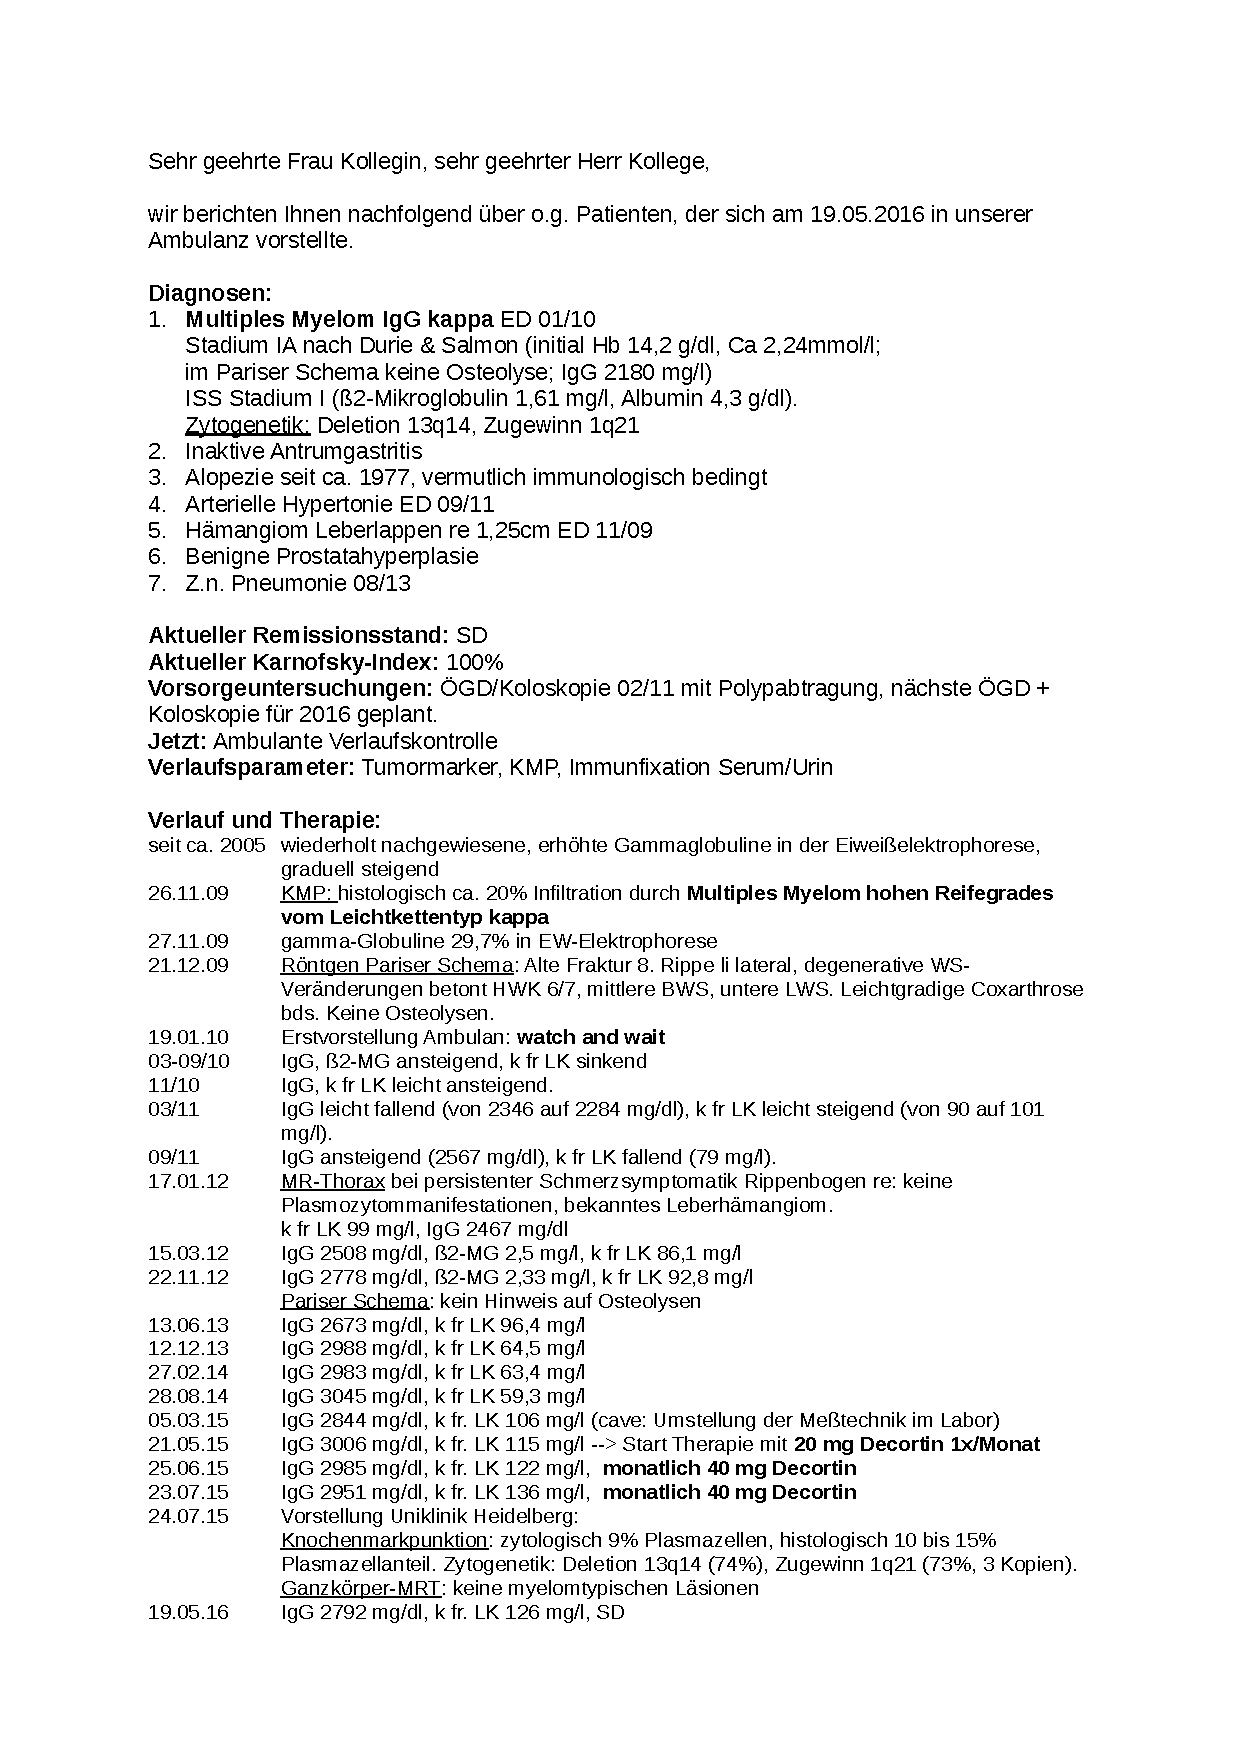
\includegraphics[width=0.85\linewidth]{figures/Brief001_1}
	\caption{First page of one exemplary physician letter. At the top is a short and general greeting. Next one can see a list of several diagnosis with additional information about medical parameters. The next section includes more medical parameters not related to one specific diagnosis. Then the therapy history is shown, including medical disease parameters over time and special results obtained e.g. during an MRI.}
	\label{fig:letter_first_page}
\end{figure}

\begin{figure}[h]
	\centering
	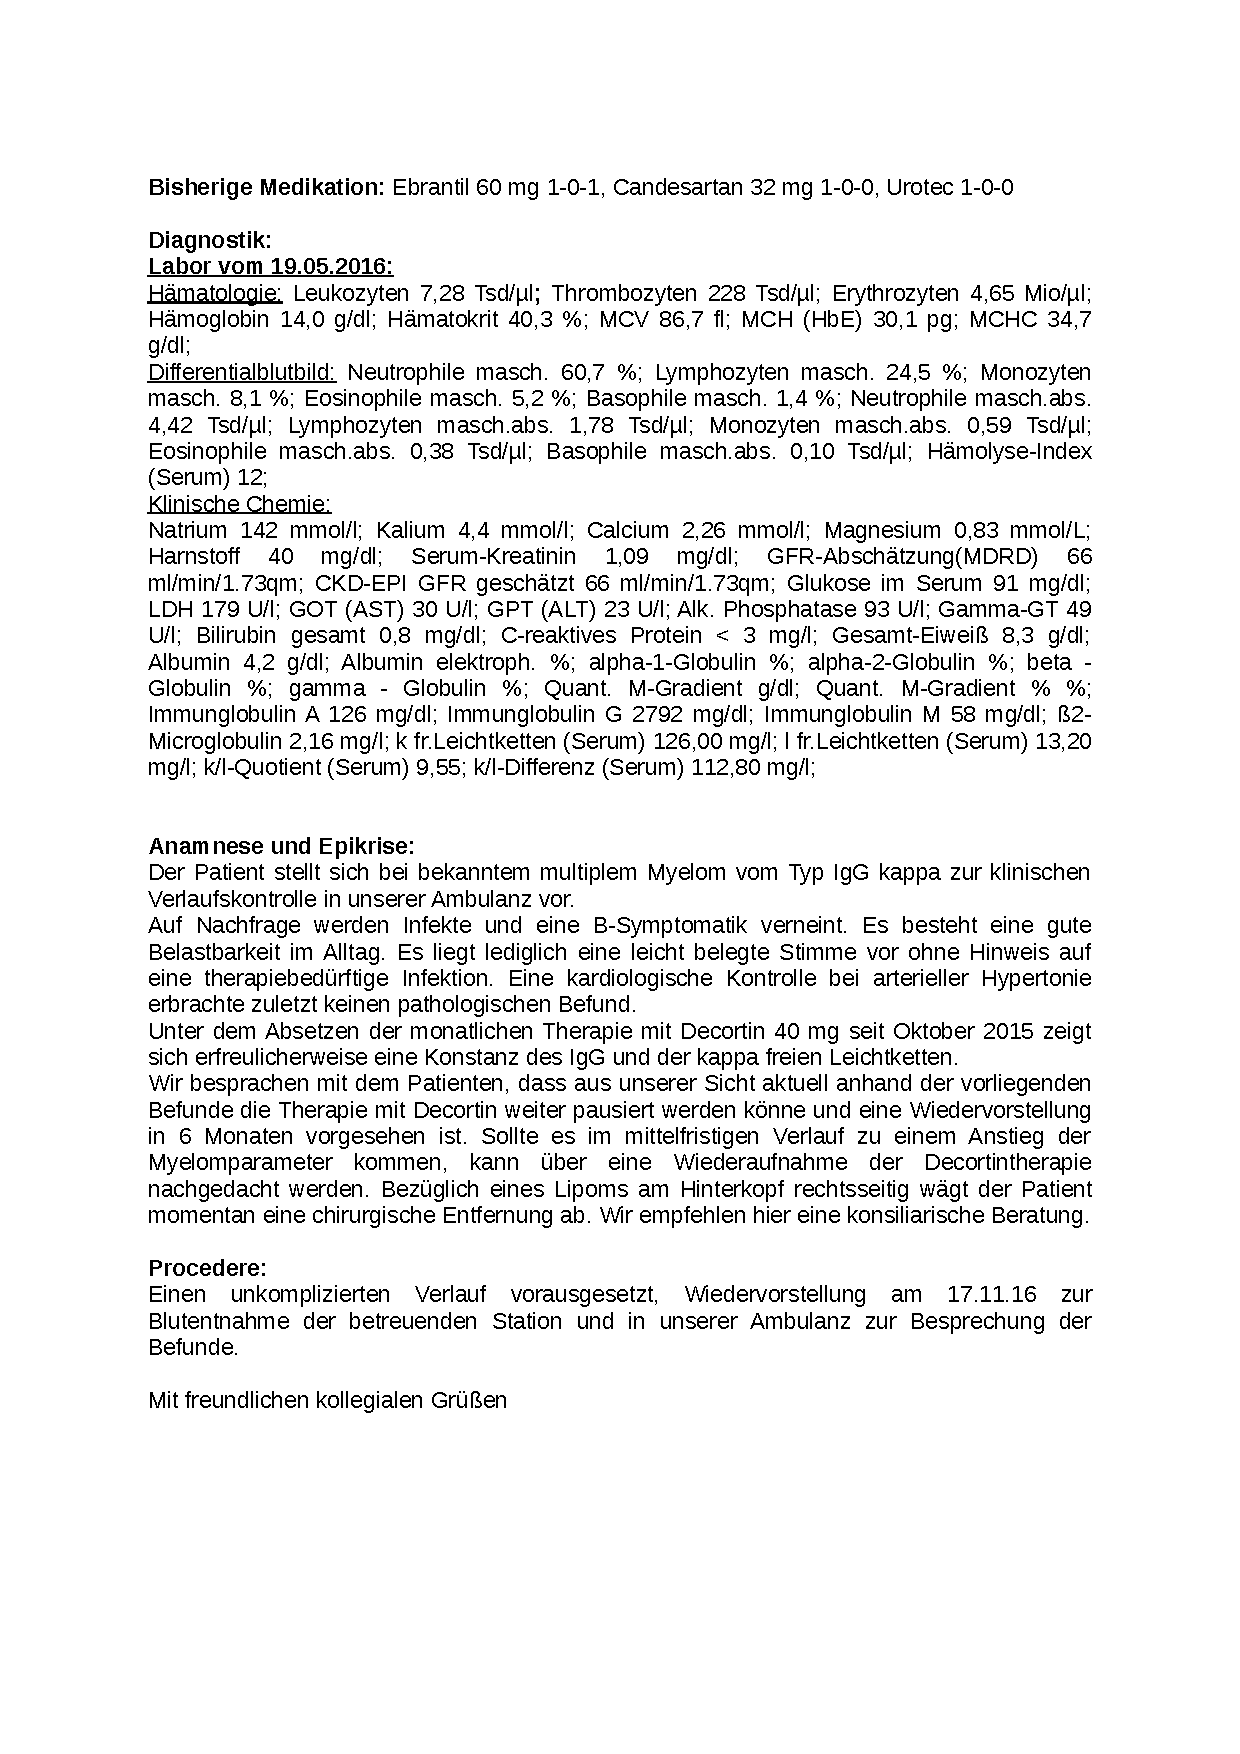
\includegraphics[width=0.87\linewidth]{figures/Brief001_2}
	\caption{Second page of one exemplary physician letter. At the top one can see the so far used medication. The next section describes detailed laboratory examination results of blood counts. Then the current anamnesis is shown, where e.g. the patient's current complaints are listed. The subsequent paragraph discusses the procedure for the next six months. Finally ``goodbye regards'' are given.}
	\label{fig:letter_second_page}
\end{figure}

\begin{figure}[h]
	\centering
	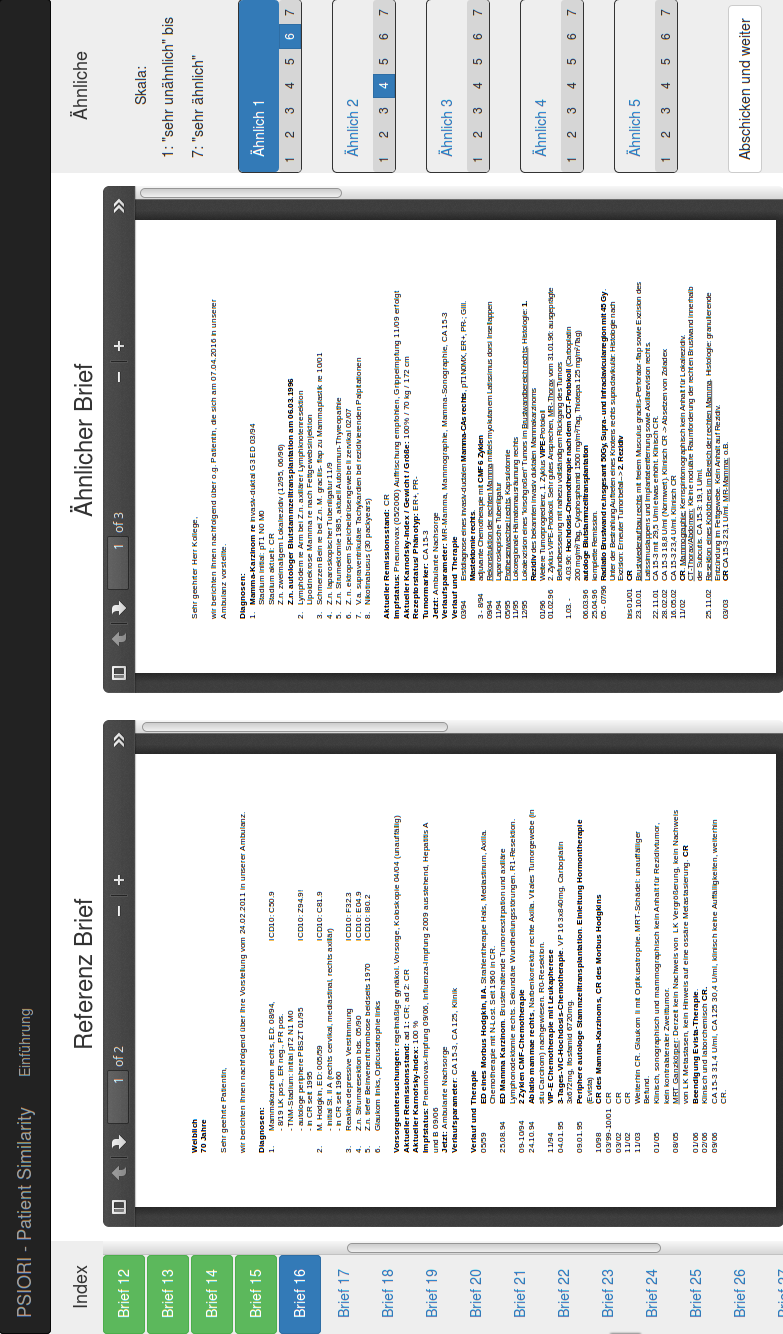
\includegraphics[width=0.85\linewidth]{figures/webexperiment_screenshot}
	\caption{Screenshot of the whole webpage, where subjects conducted the experiment.}
	\label{fig:whole_webexperiment}
\end{figure}


\begin{figure}[h]
	\centering
	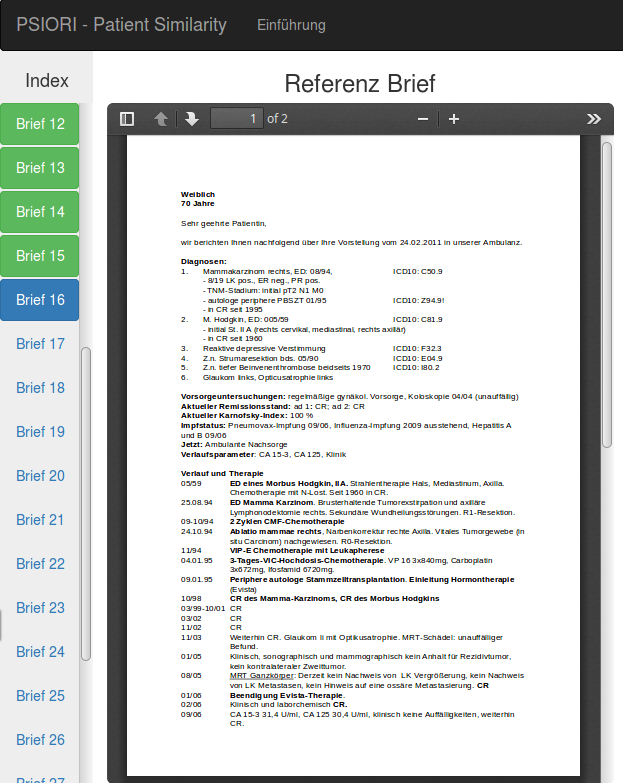
\includegraphics[width=0.9\linewidth]{figures/webexperiment_screenshot_left}
	\caption{Screenshot of the left part of the webpage, where subjects conducted the experiment. In the left column the different reference letters can be selected. The chosen reference letter is displayed right of this column.}
	\label{fig:webexperiment_left}
\end{figure}

\begin{figure}[h]
	\centering
	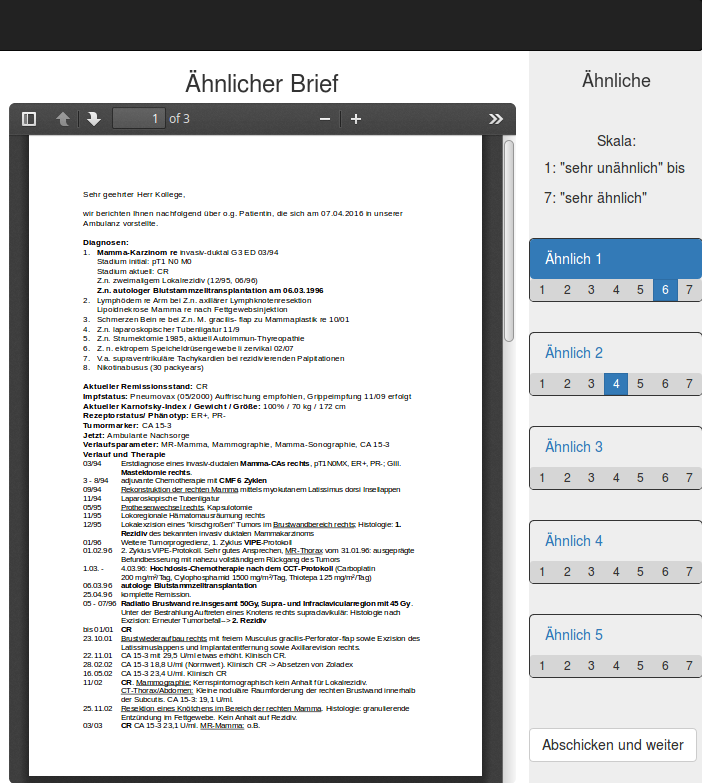
\includegraphics[width=0.9\linewidth]{figures/webexperiment_screenshot_right}
	\caption{Screenshot of the right part of the webpage, where subjects conducted the experiment. In the right column the different comparison letters can be selected and rated for their similarity to the current reference letter. The chosen comparison letter is displayed left of this column.}
	\label{fig:webexperiment_right}
\end{figure}

\chapter{Code}
The Python code comprising the recommender system itself and all experiments and evaluations we have done is attached to the printed version of this thesis as a hard copy on DVD. However, the dataset of physician letters is not included. Personal information of the patients might still be present despite our efforts to remove it.  Consequently, we prefer not to make this dataset publicly available.
\end{document}